\documentclass[11pt,a4paper,spanish]{book}
\usepackage{estilo_unir-1}
\hypersetup{
	colorlinks   = true,
	urlcolor     = blue,
	linkcolor    = black,
	citecolor    = red
}
\usepackage[nottoc]{tocbibind}
\usepackage{tikz}
\usetikzlibrary{arrows.meta, positioning, fit, calc}
\usepackage{listings}
\usepackage{graphicx}
\lstset{
	basicstyle=\ttfamily\footnotesize,
	breaklines=true,
	frame=single,
	backgroundcolor=\color[gray]{0.95},
	numbers=left,
	numberstyle=\tiny\color[gray]{0.5},
	keywordstyle=\color{blue},
	commentstyle=\color[gray]{0.5},
	tabsize=2
}

%---------------------------
% Datos del trabajo
%---------------------------
\subject{Pr\'{a}cticas Acad\'{e}micas Externas}
\title{Sistema de medici\'{o}n de impedancia (EIS) para cuantificaci\'{o}n de Candida albicans --- Fase 3}
\author{Andr\'{e}s Alexandro Tapia Flores}
\profesor{Universidad Internacional de la Rioja (UNIR)}
\date{Abril 2026}

\begin{document}
\renewcommand{\listfigurename}{\'{I}ndice de figuras}
\renewcommand{\contentsname}{\'{I}ndice de contenidos}
\renewcommand{\figurename}{Figura}
\renewcommand{\tablename}{Tabla}
\setlength{\headheight}{26pt}

\maketitle
\frontmatter
\tableofcontents

\chapter{Resumen}
En esta tercera fase se implementa la adquisici\'{o}n y visualizaci\'{o}n de datos EIS en tiempo real sobre una arquitectura completamente simulada, debido a la indisponibilidad temporal del hardware f\'{i}sico (ESP32 + AD5933). El sistema integra una tarjeta de adquisici\'{o}n serial virtual, un backend as\'{i}ncrono en Python para recolecci\'{o}n y retransmisi\'{o}n, y una interfaz web en React para representaci\'{o}n en vivo mediante diagramas de Bode y Nyquist.

Se validan tiempos de respuesta de comandos, rendimiento de barrido y consistencia de flujo de datos extremo a extremo. Adem\'{a}s, se expone en interfaz la salida del clasificador cu\'{a}ntico para comparar en tiempo real su predicci\'{o}n frente al clasificador cl\'{a}sico.

\vspace{0.5cm}
{\bf Palabras clave:} adquisici\'{o}n en tiempo real, simulaci\'{o}n serial, bode, nyquist, websocket, interfaz web

\mainmatter

\chapter{Introducci\'{o}n}

La Fase~3 del proyecto se enfoca en cubrir el entregable de adquisici\'{o}n y visualizaci\'{o}n en tiempo real. En el reto original, el backend deb\'{i}a consumir datos provenientes del ESP32 con firmware Arduino, pero durante esta iteraci\'{o}n no se dispone del equipo de laboratorio para validar en sitio.

Para mantener el avance funcional del sistema, se defini\'{o} una tarjeta de adquisici\'{o}n simulada que preserva el mismo contrato de comunicaci\'{o}n serial (comandos y mensajes JSON). De esta forma, todo el pipeline software permanece equivalente al escenario de producci\'{o}n: protocolo serial, collector as\'{i}ncrono, servidor WebSocket, dashboard de monitoreo y validaci\'{o}n del clasificador.

\section{Alcance de esta fase}
Esta fase cubre:
\begin{itemize}
	\item Simulaci\'{o}n de tarjeta de adquisici\'{o}n con puerto serial virtual y perfiles de espectro.
	\item Adquisici\'{o}n no bloqueante en backend Python con reenv\'{i}o en tiempo real.
	\item Visualizaci\'{o}n en vivo de magnitud, fase y plano de Nyquist.
	\item Publicaci\'{o}n de predicci\'{o}n cu\'{a}ntica y comparaci\'{o}n con modelo cl\'{a}sico en la UI.
	\item Medici\'{o}n de latencias de protocolo y rendimiento de barrido.
\end{itemize}


\chapter{Objetivos}

\section{Objetivo general}
Implementar y validar la adquisici\'{o}n y visualizaci\'{o}n de datos EIS en tiempo real mediante una arquitectura software completa basada en simulaci\'{o}n serial del ESP32/AD5933.

\section{Objetivos espec\'{i}ficos}
\begin{itemize}
	\item Construir un emulador de tarjeta de adquisici\'{o}n con protocolo serial compatible con el firmware original.
	\item Implementar reconexi\'{o}n y consumo as\'{i}ncrono de datos en el Collector.
	\item Habilitar una interfaz de operaci\'{o}n en tiempo real con controles de configuraci\'{o}n, calibraci\'{o}n y barrido.
	\item Representar curvas Bode y Nyquist en actualizaci\'{o}n continua por punto recibido.
	\item Mostrar en la interfaz la salida del clasificador cu\'{a}ntico y su comparaci\'{o}n con clasificador cl\'{a}sico.
	\item Evaluar latencia de comandos y frecuencia de adquisici\'{o}n efectiva.
\end{itemize}


\chapter{Arquitectura de adquisici\'{o}n en tiempo real}

\section{Dise\~{n}o general de la simulaci\'{o}n}

La implementaci\'{o}n se apoya en tres procesos independientes: tarjeta simulada, backend y cliente web. La Figura~\ref{fig:arquitectura-fase3} resume los m\'{o}dulos y enlaces de comunicaci\'{o}n.

\begin{figure}[ht]
	\centering
	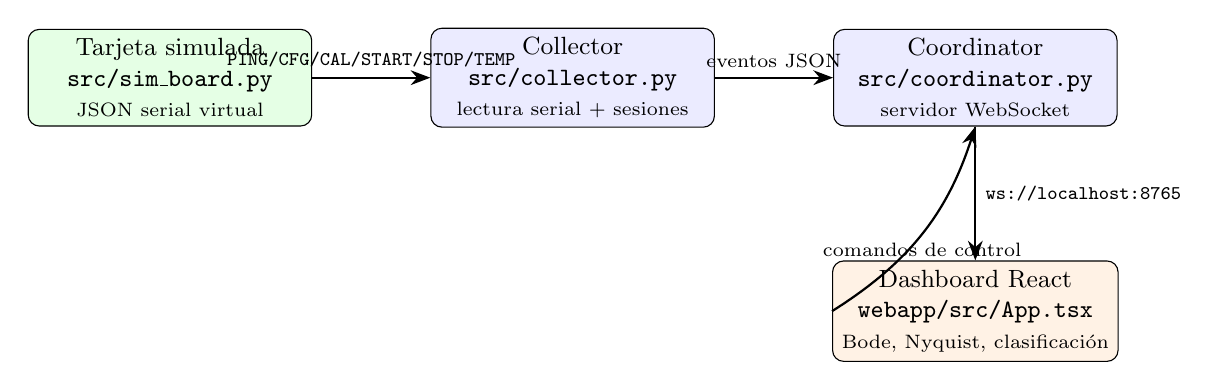
\begin{tikzpicture}[
		node distance=1.7cm and 1.5cm,
		block/.style={rectangle, draw, rounded corners, fill=blue!8, minimum width=3.6cm, minimum height=1.2cm, align=center, font=\small},
		arrow/.style={-{Stealth[length=2.5mm]}, thick}
		]
		\node[block, fill=green!10] (sim) {Tarjeta simulada\\\texttt{src/sim\_board.py}\\\scriptsize JSON serial virtual};
		\node[block, right=of sim] (collector) {Collector\\\texttt{src/collector.py}\\\scriptsize lectura serial + sesiones};
		\node[block, right=of collector] (coord) {Coordinator\\\texttt{src/coordinator.py}\\\scriptsize servidor WebSocket};
		\node[block, below=of coord, fill=orange!10] (ui) {Dashboard React\\\texttt{webapp/src/App.tsx}\\\scriptsize Bode, Nyquist, clasificaci\'{o}n};

		\draw[arrow] (sim) -- node[above, font=\scriptsize]{\texttt{PING/CFG/CAL/START/STOP/TEMP}} (collector);
		\draw[arrow] (collector) -- node[above, font=\scriptsize]{eventos JSON} (coord);
		\draw[arrow] (coord) -- node[right, font=\scriptsize]{\texttt{ws://localhost:8765}} (ui);
		\draw[arrow] (ui.west) to[bend right=20] node[below, font=\scriptsize]{comandos de control} (coord.south);
	\end{tikzpicture}
	\caption[Arquitectura de adquisici\'{o}n en tiempo real]{Arquitectura de Fase~3 en modo simulado. Fuente: elaboraci\'{o}n propia.}
	\label{fig:arquitectura-fase3}
\end{figure}

\section{Comandos y eventos operativos}

La Tabla~\ref{tab:comandos-fase3} resume el conjunto de comandos utilizados durante adquisici\'{o}n y monitoreo.

\begin{table}[ht]
	\centering
	\begin{tabular}{l l p{7.5cm}}
		\hline\hline
		Comando & Formato                         & Uso en Fase 3                                                   \\ [0.5ex]
		\hline
		PING    & \texttt{PING}                   & Verifica conectividad serial y estado del enlace simulado.      \\
		CFG     & \texttt{CFG:fmin,fmax,n,settle} & Define rango de frecuencias y densidad de muestreo del barrido. \\
		CAL     & \texttt{CAL:R}                  & Ajusta factor de ganancia y fase de referencia para el barrido. \\
		START   & \texttt{START}                  & Inicia barrido completo con publicaci\'{o}n punto a punto.      \\
		STOP    & \texttt{STOP}                   & Interrumpe barrido en curso y cierra sesi\'{o}n activa.         \\
		TEMP    & \texttt{TEMP}                   & Recupera temperatura instant\'{a}nea reportada por la tarjeta.  \\
		\hline
	\end{tabular}
	\caption[Comandos usados en adquisici\'{o}n]{Comandos del protocolo operativo durante la adquisici\'{o}n en tiempo real. Fuente: elaboraci\'{o}n propia.}
	\label{tab:comandos-fase3}
\end{table}

\section{Flujo temporal por barrido}

Para cada barrido, el flujo se ejecuta en el siguiente orden:

\begin{enumerate}
	\item La UI env\'{i}a \texttt{start} por WebSocket, incluyendo etiqueta esperada (0 o 1).
	\item El backend transmite \texttt{START} a la tarjeta simulada por serial.
	\item La tarjeta publica \texttt{sweep\_start} y posteriormente una trama \texttt{data} por cada frecuencia.
	\item El collector reenv\'{i}a cada punto a la UI, actualizando gr\'{a}ficas en tiempo real.
	\item Al recibir \texttt{sweep\_done}, el collector calcula clasificaci\'{o}n y publica el evento \texttt{analysis}.
\end{enumerate}


\chapter{Visualizaci\'{o}n en tiempo real}

\section{Dise\~{n}o de la interfaz web}

El dashboard implementado en React integra cuatro bloques funcionales:
\begin{itemize}
	\item \textbf{Control de adquisici\'{o}n}: configuraci\'{o}n de barrido, calibraci\'{o}n y acciones de operaci\'{o}n.
	\item \textbf{Monitoreo de estado}: conexi\'{o}n, temperatura y progreso de puntos recibidos.
	\item \textbf{Visualizaci\'{o}n EIS}: Bode de magnitud, Bode de fase y Nyquist.
	\item \textbf{Clasificaci\'{o}n}: probabilidad cu\'{a}ntica, probabilidad cl\'{a}sica y validaci\'{o}n contra etiqueta esperada.
\end{itemize}

\section{Ejemplo de trazado Bode y Nyquist}

La Tabla~\ref{tab:muestra-candida} presenta puntos representativos de un barrido simulado con etiqueta esperada \texttt{1} (candida).

\begin{table}[ht]
	\centering
	\scriptsize
	\begin{tabular}{r r r r r r}
		\hline\hline
		$i$ & $f$ (Hz)   & $|Z|$ ($\Omega$) & $\phi$ (grados) & $\mathrm{Re}(Z)$ ($\Omega$) & $\mathrm{Im}(Z)$ ($\Omega$) \\ [0.5ex]
		\hline
		0   & 1000.0     & 231.7808         & -13.6895        & 225.1964                    & -54.8534                    \\
		4   & 1603.7187  & 226.4788         & -8.9712         & 223.7082                    & -35.3167                    \\
		8   & 2571.9138  & 224.4571         & -5.7741         & 223.3183                    & -22.5818                    \\
		12  & 4124.6264  & 223.7234         & -3.7627         & 223.2411                    & -14.6816                    \\
		16  & 6614.7406  & 221.6339         & -2.4827         & 221.4259                    & -9.6005                     \\
		20  & 10608.1836 & 221.4077         & -1.6335         & 221.3177                    & -6.3116                     \\
		24  & 17012.5428 & 222.0555         & -1.0828         & 222.0158                    & -4.1961                     \\
		28  & 27283.3338 & 220.4741         & -0.7379         & 220.4558                    & -2.8394                     \\
		32  & 43754.7938 & 219.9725         & -0.5056         & 219.9639                    & -1.9412                     \\
		36  & 70170.3829 & 220.5245         & -0.3490         & 220.5204                    & -1.3434                     \\
		39  & 100000.0   & 220.3323         & -0.2663         & 220.3300                    & -1.0242                     \\
		\hline
	\end{tabular}
	\caption[Muestra de puntos en barrido candida]{Muestra de puntos exportados durante un barrido simulado etiquetado como candida. Fuente: elaboraci\'{o}n propia a partir de sesi\'{o}n \texttt{session\_20260417\_054612\_940592}.}
	\label{tab:muestra-candida}
\end{table}

La Figura~\ref{fig:trazos-fase3} sintetiza de forma conceptual la representaci\'{o}n de Bode y Nyquist obtenida en tiempo real.

\begin{figure}[ht]
	\centering
	\resizebox{\textwidth}{!}{%
		\begin{tikzpicture}[x=0.2cm,y=0.03cm]
			\draw[thick, -{Stealth[length=2.5mm]}] (0,0) -- (52,0) node[right]{\scriptsize Punto de frecuencia};
			\draw[thick, -{Stealth[length=2.5mm]}] (0,0) -- (0,130) node[above]{\scriptsize Escala relativa};

			\draw[blue, thick] plot coordinates {
					(1,116) (6,103) (11,97) (16,93) (21,89) (26,87) (31,86) (36,85) (41,84) (46,84) (50,84)
				};
			\draw[red, thick, dashed] plot coordinates {
					(1,102) (6,85) (11,73) (16,64) (21,57) (26,52) (31,48) (36,45) (41,43) (46,41) (50,40)
				};

			\node[blue] at (42,112) {\scriptsize $|Z|$ Bode};
			\node[red] at (40,70) {\scriptsize Fase Bode};

			\begin{scope}[shift={(63,0)}, x=0.03cm, y=0.045cm]
				\draw[thick, -{Stealth[length=2.5mm]}] (0,0) -- (380,0) node[right]{\scriptsize $\mathrm{Re}(Z)$};
				\draw[thick, -{Stealth[length=2.5mm]}] (0,0) -- (0,140) node[above]{\scriptsize $-\mathrm{Im}(Z)$};
				\draw[green!70!black, thick] plot coordinates {
						(225,55) (224,35) (223,23) (222,15) (221,10) (221,6) (220,4) (220,3) (220,2) (220,1)
					};
				\node[green!60!black] at (250,120) {\scriptsize Nyquist};
			\end{scope}
		\end{tikzpicture}
	}%
	\caption[Representaci\'{o}n conceptual de trazos en tiempo real]{Representaci\'{o}n conceptual de trazos Bode y Nyquist desplegados durante adquisici\'{o}n en vivo. Fuente: elaboraci\'{o}n propia.}
	\label{fig:trazos-fase3}
\end{figure}


\chapter{Pruebas y resultados}

\section{Escenario de validaci\'{o}n}

La validaci\'{o}n se ejecut\'{o} con tres procesos:
\begin{itemize}
	\item \texttt{make sim-board}
	\item \texttt{make server-sim}
	\item \texttt{make webapp}
\end{itemize}

El backend y la tarjeta simulada se verificaron tambi\'{e}n con una prueba automatizada por WebSocket, registrando latencias por comando y cierre completo de barrido con publicaci\'{o}n de an\'{a}lisis.

\section{Latencia por comando}

La Tabla~\ref{tab:latencias-fase3} resume los tiempos medidos para un ciclo completo de operaci\'{o}n.

\begin{table}[ht]
	\centering
	\begin{tabular}{l r l}
		\hline\hline
		Operaci\'{o}n                & Tiempo medido & Observaci\'{o}n                                   \\ [0.5ex]
		\hline
		PING                         & 3.22 ms       & Respuesta inmediata de enlace serial+WS           \\
		CFG                          & 2.58 ms       & Actualizaci\'{o}n de configuraci\'{o}n de barrido \\
		CAL                          & 2.45 ms       & Confirmaci\'{o}n de calibraci\'{o}n               \\
		TEMP                         & 2.33 ms       & Lectura de temperatura instant\'{a}nea            \\
		START $\rightarrow$ ANALYSIS & 419.96 ms     & Barrido de 40 puntos + clasificaci\'{o}n          \\
		\hline
	\end{tabular}
	\caption[Latencias medidas del protocolo]{Latencias medidas para comandos principales del flujo de adquisici\'{o}n. Fuente: elaboraci\'{o}n propia.}
	\label{tab:latencias-fase3}
\end{table}

\section{Rendimiento de adquisici\'{o}n}

Se registraron dos barridos de 40 puntos (candida/control) para evaluar consistencia temporal:
\begin{itemize}
	\item Barrido candida: 0.4118 s totales, 94.70 puntos/s.
	\item Barrido control: 0.4089 s totales, 95.39 puntos/s.
\end{itemize}

Los resultados muestran una tasa sostenida cercana a 95 puntos/s, suficiente para visualizaci\'{o}n continua sin bloqueos perceptibles en la UI.

\section{Clasificaci\'{o}n mostrada en UI}

La Tabla~\ref{tab:clasificacion-ui} resume los resultados publicados en tiempo real en la interfaz para dos sesiones consecutivas.

\begin{table}[ht]
	\centering
	\scriptsize
	\begin{tabular}{l c c c c c}
		\hline\hline
		Sesi\'{o}n & Etiqueta esperada & Prob. cu\'{a}ntica & Label Q & Prob. cl\'{a}sica & Label C \\ [0.5ex]
		\hline
		S1         & 1                 & 0.658004           & 1       & 0.949788          & 1       \\
		S2         & 0                 & 0.407482           & 0       & 0.080267          & 0       \\
		\hline
	\end{tabular}
	\caption[Resultado de clasificaci\'{o}n en interfaz]{Comparaci\'{o}n de salida cu\'{a}ntica y cl\'{a}sica en interfaz al finalizar cada barrido (S1: \texttt{...054612\_940592}, S2: \texttt{...054613\_366924}). Fuente: elaboraci\'{o}n propia.}
	\label{tab:clasificacion-ui}
\end{table}

\begin{figure}[ht]
	\centering
	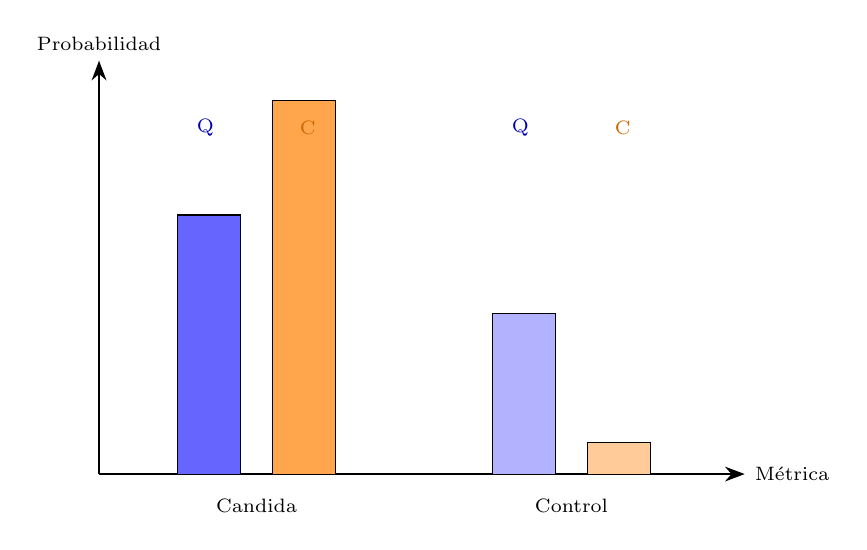
\begin{tikzpicture}[x=1.0cm,y=5cm]
		\draw[thick, -{Stealth[length=2.5mm]}] (0,0) -- (8.2,0) node[right]{\scriptsize M\'{e}trica};
		\draw[thick, -{Stealth[length=2.5mm]}] (0,0) -- (0,1.05) node[above]{\scriptsize Probabilidad};

		\draw[fill=blue!60] (1.0,0) rectangle (1.8,0.6580);
		\draw[fill=orange!70] (2.2,0) rectangle (3.0,0.9498);
		\node[align=center, font=\scriptsize] at (2.0,-0.08) {Candida};

		\draw[fill=blue!30] (5.0,0) rectangle (5.8,0.4075);
		\draw[fill=orange!40] (6.2,0) rectangle (7.0,0.0803);
		\node[align=center, font=\scriptsize] at (6.0,-0.08) {Control};

		\node[blue!70!black, font=\scriptsize] at (1.35,0.88) {Q};
		\node[orange!80!black, font=\scriptsize] at (2.65,0.88) {C};
		\node[blue!70!black, font=\scriptsize] at (5.35,0.88) {Q};
		\node[orange!80!black, font=\scriptsize] at (6.65,0.88) {C};
	\end{tikzpicture}
	\caption[Comparaci\'{o}n de probabilidades por sesi\'{o}n]{Comparaci\'{o}n visual de probabilidades publicadas por el clasificador cu\'{a}ntico (Q) y cl\'{a}sico (C) en dos sesiones de prueba. Fuente: elaboraci\'{o}n propia.}
	\label{fig:probabilidades-fase3}
\end{figure}


\chapter{Conclusiones}

En esta fase se alcanz\'{o} el objetivo de adquisici\'{o}n y visualizaci\'{o}n en tiempo real bajo un entorno totalmente simulado, manteniendo el contrato t\'{e}cnico del protocolo serial definido en fases previas.

Los principales resultados son:
\begin{itemize}
	\item La tarjeta simulada permite reproducir comandos, telemetr\'{i}a EIS y comportamiento temporal del flujo de barrido.
	\item El backend asincr\'{o}nico procesa y distribuye puntos de manera continua, con latencias de comando inferiores a 4 ms.
	\item El frontend representa en tiempo real curvas Bode y Nyquist con estabilidad visual y sin bloqueos.
	\item La UI incorpora validaci\'{o}n expl\'{i}cita del clasificador cu\'{a}ntico frente al cl\'{a}sico, incluyendo comparaci\'{o}n con etiqueta esperada.
	\item Se garantiza una base robusta para la Fase~4, centrada en persistencia, metadatos, exportaci\'{o}n y trazabilidad de sesiones.
\end{itemize}

\begin{thebibliography}{99}
	\bibitem[Analog Devices(2017)]{ad5933ds} Analog Devices (2017). \emph{AD5933: 1 MSPS, 12-Bit Impedance Converter, Network Analyzer}. Datasheet Rev.~F.
	\bibitem[pyserial(2020)]{pyserial} Liechti, C. (2020). pySerial 3.5 Documentation. \url{https://pyserial.readthedocs.io/}
	\bibitem[Python Software Foundation(2026)]{pythonasyncio} Python Software Foundation (2026). \emph{asyncio --- Asynchronous I/O}. \url{https://docs.python.org/3/library/asyncio.html}
	\bibitem[websockets(2026)]{websocketslib} Aymeric Augustin et al. (2026). \emph{websockets 16 Documentation}. \url{https://websockets.readthedocs.io/}
	\bibitem[Havl\'{i}\v{c}ek et al.(2019)]{havlicek2019} Havl\'{i}\v{c}ek, V., C\'{o}rcoles, A. D., Temme, K., Harrow, A. W., Kandala, A., Chow, J. M., \& Gambetta, J. M. (2019). Supervised learning with quantum-enhanced feature spaces. \emph{Nature}, 567(7747), 209--212.
\end{thebibliography}

\end{document}
